\chapter{Introdu\c{c}\~ao}
Segundo a \textit{World Semiconductor Trade Statistics}, cada pessoa no planeta comprou uma média de 111 chips ou circuitos integrados (ICs) em 2016. O uso desses dispositivos semicondutores está crescendo cinco vezes a taxa de crescimento da população humana \cite{Sameer}. \par
\noindent Natural que haja uma busca por dispositivos que possibilitem maior densidade de transistores, bem como menor dissipação de energia na forma de calor. Transistores de Nitreto de Gálio e Carbeto de Silício vem se mostrando como alternativa ao cenário atual, com Silício. São bons chaveadores em alta frequência além baixa resistência quando ligados \cite{lidow_rooij_strydom_reusch_glaser_2020}. 

\section{Energia renovavel - Solar}
Intro
\subsection{Pisco de Luz}
Falar sobre a organização. 
\subsection{Sistema de iluminação}

\section{Transistores em circuitos de potência}
\subsection{Transistores de potência baseados em Silício}
Os transistores de potência baseados em silício, tiveram sua eficiência e o custo do gerenciamento de energia melhorado continuamente nas ultimas decadas. Inovações em estruturas do transistor acompanharam a crescente necessidade de equipamentos eletrônicos em nossas vidas diárias. No entanto, a taxa de melhoria diminuiu bastante, uma vez que ,assintoticamente, se aproxima de seus limites teóricos. \cite{lidow_rooij_strydom_reusch_glaser_2020}

\subsection{Transistor baseados em Nitreto de Gálio (GaN)}
Dispositivos baseados em Nitreto de Gálio (GaN) apareceram pela primeira vez em cerca de 2004, como transistores de radiofrequência (RF) feitos pela Eudyna Corporation do Japão. Usando GaN em substratos de carbeto de silício (SiC), a Eudyna produziu transistores projetados para o mercado de RF, com sucesso \cite{Alex}. Porém, não só do ponto de vista de RF há vantagens em utilizar GaN, há vantagens também em eletrônica de potência. As caracteristicas dos dispositivos baseados em Nitreto de Gálio podem ser vistas na comparação da Tabela \ref{t_materiais}.

\begin{table}[!htb]
\centering
\caption{Comparação entre propriedades dos materiais \cite{lidow_rooij_strydom_reusch_glaser_2020}}
\begin{tabular}{lllll}
\hline
Parâmetro           &                & Si    & SiC   & GaN \\ \hline
Banda de Gap $E_g$& $(eV)$             & 1,12  & 3,39  & 3,26\\
Campo Elétrico crítico $E_{Crit}$ &$(MV/cm)$   & 0,23  & 3,3   & 2,2\\
Mobilidade dos elétrons $\mu_n$ &$(cm^2/V.s)$& 1400  & 1500  & 950\\
Permissividade $\varepsilon_r$ &     & 11,8  & 9     & 9,7\\
Condutividade térmica $\lambda$& $(W/cm.K)$     & 1,5   & 1,3   & 3,8\\ \hline
\end{tabular}
\label{t_materiais}
\end{table}

\subsubsection{Banda de Gap $(E_g)$}
A banda de Gap de um semicondutor está relacionado à força das ligações químicas entre os átomos na rede. Essas ligações mais fortes significam que é mais difícil para um elétron saltar de um nível para o próximo. Entre as muitas consequências estão correntes de fuga intrínsecas mais baixas e maiores temperaturas de operação para semicondutores de gap maior. Com base nos dados da Tabela \ref{t_materiais}, GaN e SiC têm banda de Gap maiores do que o silício. \cite{lidow_rooij_strydom_reusch_glaser_2020}

\subsubsection{Resistência quando ligado $(R_{DS_{(on)}})$}
A resistência teórica, em Ohms ($\Omega$), será dada pela equação \ref{RdsOn}. \cite{lidow_rooij_strydom_reusch_glaser_2020}
\begin{equation}
    R_{DS_{(on)}} = \frac{W_{drift}}{q.\mu_n .N_D}
    \label{RdsOn}
\end{equation}
A resistência, quando relacionada com o Campo Elétrico Crítico $(E_g)$ será dada por \ref{RdsOnEg}. \cite{lidow_rooij_strydom_reusch_glaser_2020}
\begin{equation}
    R_{DS_{(on)}} = \frac{4.V^2_{BR}}{\varepsilon_o .\varepsilon_r . E^3_{crit}}
    \label{RdsOnEg}
\end{equation}
A equação dada por \ref{RdsOnEg} está representada no gráfico da Figura \ref{FigRDSon}.
\begin{figure}[H]
\caption{Resistência $R_{DS_(on)}$ vs capacidade de bloquear tensão para dispositivos Si, SiC, and GaN \cite{lidow_rooij_strydom_reusch_glaser_2020}}
 \centering % para centralizarmos a figura
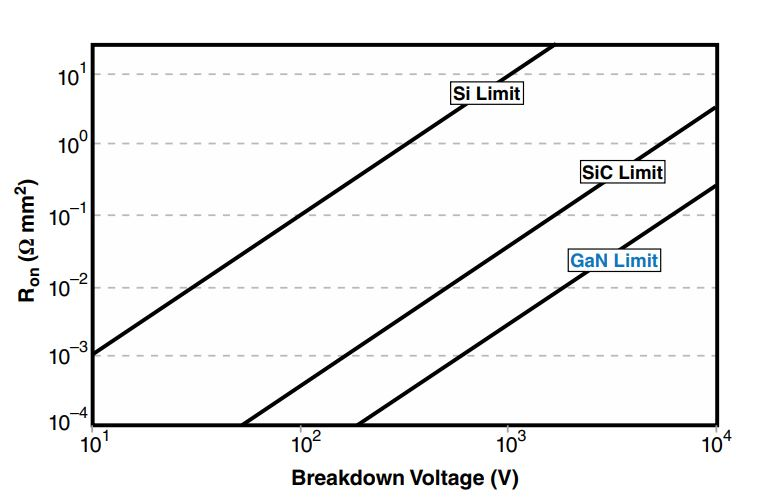
\includegraphics[width=14cm]{figuras/5.JPG} 
\label{FigRDSon}
\end{figure}
\noindent Junto com a baixa resistência $R_{DS_(on)}$, há o benefício de conseguir trabalhar em frequências mais altas que IGBTs com potências relativamente altas, como mostra a Figura \ref{FigComparison}. 
\begin{figure}[H]
\caption{Potência vs Frequência. \cite{Sameer}}
 \centering % para centralizarmos a figura
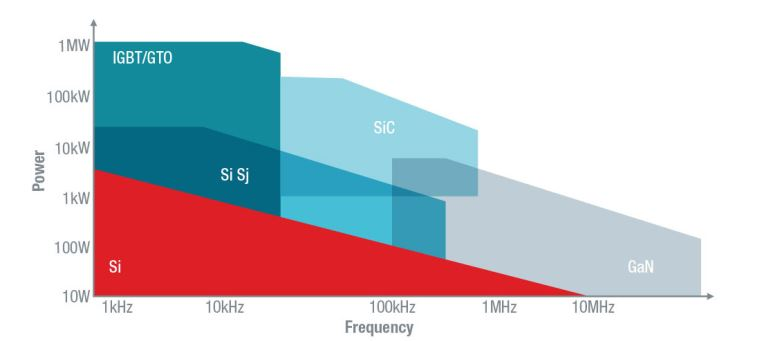
\includegraphics[width=15cm]{figuras/6.JPG} 
\label{FigComparison}
\end{figure}





